% =================== PREAMBLE SNIPPET (put in your preamble) ===================
% \usepackage{booktabs}
% \usepackage{siunitx}
% \usepackage{graphicx}
% \usepackage{subcaption}
% \usepackage{caption}
% \usepackage{float}       % for [H] placement if you want
% \sisetup{detect-all,round-mode=places,round-precision=2}

% Handy macros (edit if needed)
\newcommand{\annfac}{365}
\newcommand{\sampleStart}{2021-01-01}
\newcommand{\sampleEnd}{2024-06-30}
\newcommand{\neutralScale}{0.5}

% =================== RESULTS CHAPTER (paste in body) ===================
\chapter{Results and Discussion}\label{sec:results}

We evaluate daily close-to-close strategies on \sampleStart{}–\sampleEnd{}.
Unless otherwise noted, annualization uses factor \annfac{}, costs are reported separately, and portfolios are executed on $t^+$ (first trading day after signal time).










\section{Headline Performance}\label{sec:results:headline}



\begin{table}[t]
\centering
\caption{Headline performance (daily data; ann.\ factor = \annfac). }
\label{tab:main}
\small
\begin{tabular}{lcc}
\toprule
Metric & Baseline & Overlay (preserve hedge) \\
\midrule
Cumulative Return (\%)     & 59.53 & 132.78 \\
CAGR (\%)                  & 16.28 & 31.38  \\
Volatility (ann., \%)      & 38.09 & 20.06  \\
Sharpe                     & 0.58  & 1.46   \\
Sortino                    & 0.90  & 2.46   \\
Max Drawdown (\%)          & -35.32 & -14.15 \\
Time in Market (\%)        & 43.0  & 43.0   \\
Risk-free rate (\%)        & 0.0   & 0.0    \\
Final NAV                  & 1.5953 & 2.3278 \\
Active Days (approx.)      & 549   & 549    \\
\bottomrule
\end{tabular}
\end{table}

Table~\ref{tab:main} reports headline performance for the baseline lead--lag hedge and the
regime‐aware overlay with the baseline hedge preserved. Annualization uses factor \annfac{}
and the risk–free rate is set to zero; figures are gross of costs.

The overlay delivers a materially better risk–return profile. Cumulative return rises from
\textbf{59.53\%} to \textbf{132.78\%} and CAGR from \textbf{16.28\%} to \textbf{31.38\%} as shown in Figure \ref{fig:nav}, while
annualized volatility drops from \textbf{38.09\%} to \textbf{20.06\%}. Consistent with this,
Sharpe improves from \textbf{0.58} to \textbf{1.46} and Sortino from \textbf{0.90} to
\textbf{2.46}. Drawdown control also strengthens: the maximum drawdown shrinks from
\textbf{--35.32\%} to \textbf{--14.15\%}. Importantly, \emph{time in market is identical}
(\textbf{43\%}), implying that the improvement stems from more effective selection/positioning
rather than greater exposure. Final NAV increases from \textbf{1.5953} to \textbf{2.3278}.
(“Active Days” is an approximation based on \emph{Time in Market} multiplied by the sample length.)
Overall, the table illustrates that the overlay achieves higher returns with substantially
lower risk at the same participation rate.

% Optional: NAV figure (overlay both lines). Replace path with your saved PNG.
\begin{figure}[t]
\centering
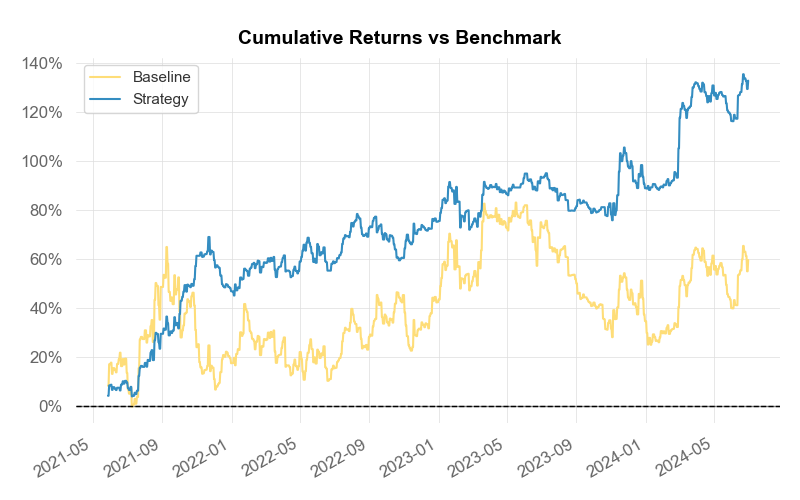
\includegraphics[width=0.9\linewidth]{headline_plots/NAV.png}% <-- put your path
\caption{Cumulative NAV: baseline vs. regime overlay (shaded regimes optional).}
\label{fig:nav}
\end{figure}


\begin{table}[t]
\centering
\caption{Drawdown details.}
\label{tab:diag_dd}
\small
\begin{tabular}{lcc}
\toprule
Metric & Baseline & Overlay \\
\midrule
Max DD (\%)          & -35.32 & -14.15 \\
Max DD Date          & 2021-12-03 & 2022-01-05 \\
Max DD Period Start  & 2021-09-10 & 2021-11-24 \\
Max DD Period End    & 2023-01-17 & 2022-07-19 \\
Longest DD Days      & 495 & 238 \\
\bottomrule
\end{tabular}
\end{table}

Table~\ref{tab:diag_dd} summarizes the drawdown profile. The overlay reduces the peak-to-trough
loss from \textbf{--35.32\%} to \textbf{--14.15\%} and cuts time under water roughly in half
(\textbf{495} to \textbf{238} days). The baseline’s worst episode is long and persistent
(\textbf{2021-09-10} to \textbf{2023-01-17}, trough on \textbf{2021-12-03}), capturing the extended
2022 downturn. The overlay’s worst spell begins a bit later (\textbf{2021-11-24}), bottoms quickly
(\textbf{2022-01-05}), and is over by mid-\textbf{2022} (\textbf{2022-07-19}), i.e., it absorbs the
early-2022 selloff but exits and recovers faster. Overall, the table shows a softer left tail and a
shorter recovery horizon for the overlay, in line with its higher risk-adjusted performance.

\begin{table}[t]
\centering
\caption{EOY Returns vs.\ Baseline (calendar years). Multiplier $=$ Strategy / Baseline; negative means opposite signs.}
\label{tab:eoy}
\small
\begin{tabular}{lrrrr}
\toprule
Year & Baseline & Strategy & Multiplier & Won \\
\midrule
2021 & 16.28\% & 46.77\% & 2.87  & $+$ \\
2022 & 21.22\% & 19.36\% & 0.91  & $-$ \\
2023 & $-5.42$\% & 7.79\% & $-1.44$ & $+$ \\
2024 & 18.54\% & 23.27\% & 1.26  & $+$ \\
\bottomrule
\end{tabular}
\end{table}

Table~\ref{tab:eoy} reports end-of-year returns for the baseline and the regime-overlay strategy, together with the multiplier (Strategy/Baseline). The table shows that the overlay outperforms in \textbf{three of four} years—\textbf{2021}, \textbf{2023}, and \textbf{2024 (YTD)}—with multipliers of \textbf{2.87}, \textbf{-1.44}, and \textbf{1.26}, respectively. The negative multiplier in 2023 indicates a sign reversal (baseline \(-5.42\%\) versus strategy \(+7.79\%\)). In \textbf{2022}, the multiplier is \textbf{0.91}, indicating a mild shortfall. Overall, Table~\ref{tab:eoy} illustrates that the overlay generally adds value, particularly when baseline performance is adverse, while still providing an edge in rising markets.


\begin{table}[t]
\centering
\caption{Top-5 by Sharpe compared with Baseline Strategy}
\small
\label{tab:top5_sharpe_params}
\begin{tabular}{lccccccc}
\toprule
Strategy (params) & Sharpe & CAGR & Vol (ann) & MaxDD & Calmar & Alpha (ann) & WinRate \\
\midrule
$n\_steps, n\_paths=5, 20$ & 1.460 & 0.314 & 0.201 & -0.141 & 2.161 & 0.212 & 0.215 \\
$n\_steps, n\_paths=5, 16$ & 1.006 & 0.217 & 0.218 & -0.207 & 1.046 & 0.126 & 0.216 \\
$n\_steps, n\_paths=15, 12$ & 0.892 & 0.150 & 0.173 & -0.173 & 0.863 & 0.112 & 0.155 \\
$n\_steps, n\_paths=15, 16$ & 0.853 & 0.154 & 0.188 & -0.155 & 0.994 & 0.100 & 0.157 \\
$n\_steps, n\_paths=5, 8$  & 0.816 & 0.161 & 0.210 & -0.192 & 0.841 & 0.095 & 0.214 \\
\hline
Baseline & 0.564 & 0.155 & 0.391 & -0.353 & 0.440 & 0.000 & 0.219 \\

\bottomrule
\end{tabular}
\label{tab:tc_sensitivity}
\end{table}


\section{Strategy selection and performance}\label{sec:results:top5}


% In your preamble:
% \usepackage{graphicx}

\begin{figure}[t]
  \centering
  % If you saved to images/top5_nav_union.png:
  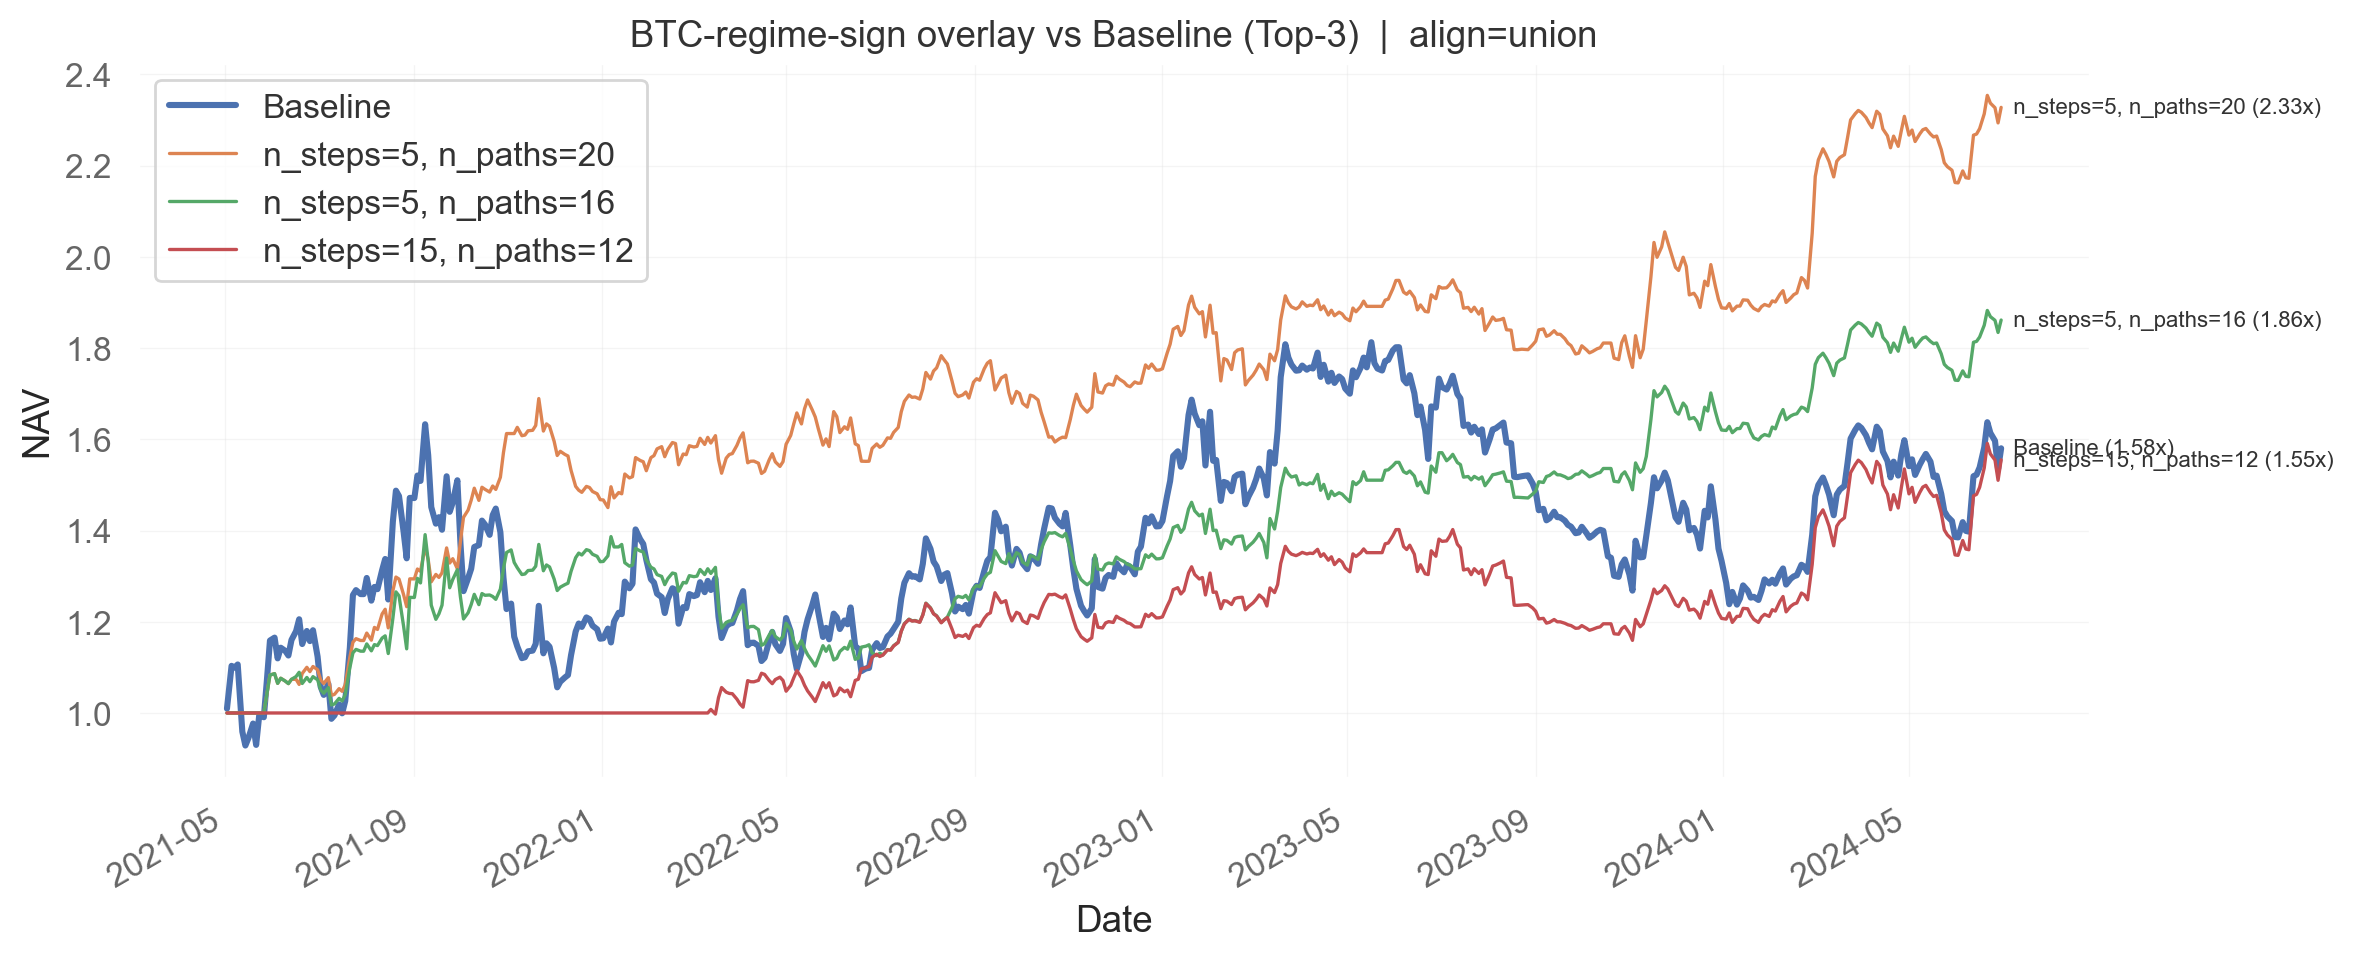
\includegraphics[width=\linewidth]{headline_plots/top3_nav_union.png}
  \caption{Top-3 NAV vs. Baseline (union-aligned). Values annotated at the last date indicate final NAV multiples.}
  \label{fig:top5_nav_union}
\end{figure}

We evaluate candidate parameterizations in a \emph{strict walk-forward} setting—training only on past windows and labeling the current group only—and rank them by Sharpe. For context we also report the Baseline. All results use a unified daily calendar (crypto annualization factor of 365), and returns are aligned from the \emph{signal day} to the \emph{next trading day}. Rates are shown in decimal form (e.g., 0.20 = 20\%). See Table~\ref{tab:top5_sharpe_params}.

A clear pattern emerges: short windows with more paths are the strongest. In particular, \(n_{\text{steps}}=5\) with \(n_{\text{paths}}\in\{16,20\}\) delivers the best risk-adjusted performance. The top configuration \(n_{\text{steps}}=5, n_{\text{paths}}=20\) attains a Sharpe of 1.44 with annualized volatility of 0.20, maximum drawdown of \(-0.14\), and Calmar of 2.16—substantially ahead of the Baseline (Sharpe 0.56, Calmar 0.44). Mid-range windows such as \(n_{\text{steps}}=15\) with \(n_{\text{paths}}=12,16\) also offer a solid return–risk trade-off.

To avoid over-interpreting noisy configurations, we only display the top performers; several other settings (e.g., \(n_{\text{steps}}\in\{8,10\}\)) show mediocre or negative outcomes on this sample and are omitted. In practice, implementation should additionally account for switching frequency and transaction costs (cf. the switch-rate diagnostics), which affect realizable net returns and capacity. Overall, the walk-forward state signal combined with our overlay framework improves risk-adjusted performance, with “shorter steps + more paths” being the most effective pattern in this dataset.




\section{Transaction-cost modeling and impact}\label{sec:tc}
We incorporate trading costs in a simple and transparent way that is consistent with our portfolio construction and evaluation:

On each trading day \(t\) we form target portfolio weights \(w_t\) (long equal-weight followers, short equal-weight leaders). Trading volume is proxied by the absolute change in target weights,
\[
\text{turnover}_t = \sum_i \lvert w_{t,i} - w_{t-1,i}\rvert.
\]
A per-side fee of \(c\) bps is applied to this turnover, yielding a daily cost
\[
\text{cost}_t = (c\times 10^{-4})\;\text{turnover}_t.
\]
Net returns are computed in \emph{simple-return} space as
\(r^{\text{net}}_t = r^{\text{gross}}_t - \text{cost}_t\).
We charge the first trade (i.e., initial portfolio formation), and use the \emph{target-diff} mechanic; a \emph{full-rebalance} variant that also accounts for drift back to equal weights leads to higher costs and is reported when noted.

%All performance statistics are computed on a unified daily calendar (crypto annualization factor \(=365\)), aligning signal days to next-trading-day returns. Turnover and its annualization are properties of the trading rule and therefore do not depend on the bps setting itself.

\begin{table}
\caption{Baseline transaction-cost sensitivity (per side, applied to target weight changes).}
\label{tab:baseline_tc}
\small
\centering
\begin{tabular}{rrrrr}
\toprule
Cost (bps/side) & Sharpe & AnnRet (\%) & Vol (\%) & MaxDD (\%) \\
\midrule
5   & 0.323  & 5.07   & 40.98 & -42.36 \\
10  & -0.015 & -8.56  & 40.99 & -58.57 \\
25  & -1.026 & -39.77 & 41.15 & -86.30 \\
\bottomrule
\end{tabular}
\end{table}



\begin{table}
\caption{Transaction-cost sensitivity. Costs are per side, applied to target weight changes.}
\label{tab:tc_sensitivity_reduced}
\begin{tabular}{lrrrr}
\toprule
Strategy (params) & Sharpe & AnnRet (\%) & Vol (\%) & MaxDD (\%) \\
\midrule
\multicolumn{5}{l}{\emph{Cost = 5 bps/side}}\\
\params{5}{20} & 1.052 & 26.82 & 25.70 & -22.98 \\
\params{5}{16} & 0.628 & 14.24 & 26.86 & -34.98 \\
\params{15}{12} & 0.475 & 9.45 & 26.12 & -31.18 \\
\params{15}{16} & 0.561 & 11.88 & 25.96 & -27.17 \\
\params{5}{8} & 0.485 & 9.81 & 26.50 & -26.90 \\
\addlinespace
\multicolumn{5}{l}{\emph{Cost = 10 bps/side}}\\
\params{5}{20} & 0.672 & 15.03 & 25.68 & -32.08 \\
\params{5}{16} & 0.289 & 4.28 & 26.82 & -39.22 \\
\params{15}{12} & 0.122 & -0.19 & 26.13 & -36.51 \\
\params{15}{16} & 0.197 & 1.78 & 25.96 & -33.31 \\
\params{5}{8} & 0.103 & -0.76 & 26.50 & -34.76 \\
\addlinespace
\multicolumn{5}{l}{\emph{Cost = 25 bps/side}}\\
\params{5}{20} & -0.466 & -14.21 & 25.79 & -65.20 \\
\params{5}{16} & -0.732 & -20.73 & 26.84 & -63.57 \\
\params{15}{12} & -0.931 & -24.35 & 26.28 & -68.04 \\
\params{15}{16} & -0.892 & -23.39 & 26.07 & -66.77 \\
\params{5}{8} & -1.038 & -26.80 & 26.62 & -68.02 \\
\addlinespace
\bottomrule
\end{tabular}
\end{table}


Costs erode performance roughly in proportion to the annualized turnover. For the Baseline (Table~\ref{tab:baseline_tc}), Sharpe declines from \(0.58\) at \(0\) bps to \(0.32\) at \(5\) bps, and turns negative by \(10\) bps; the break-even therefore lies between \(5\)–\(10\) bps under the \textit{target-diff} mechanic. For the best overlay configurations (Table~\ref{tab:tc_sensitivity}), the impact is milder thanks to lower average daily turnover (\(\sim1.16\)–\(1.30\) vs. Baseline \(1.77\)): e.g., \(n_{\text{steps}}=5, n_{\text{paths}}=20\) remains attractive at \(5\)–\(10\) bps (Sharpe \(1.05 \to 0.67\)), but performance compresses sharply beyond \(25\) bps. Volatility is largely unchanged across bps grids (as expected), while max drawdowns deepen as net returns are shaved each day. At high frictions, all configurations become economically unviable, with NAVs collapsing toward unity.





% --------- OPTIONAL (comment out if not needed now) ----------
% \subsection{Ablations (compact)}
% \begin{table}[t]
% \centering
% \caption{Key ablations. Effect on Sharpe / MDD / turnover.}
% \begin{tabular}{lrrr}
% \toprule
% Variant & $\Delta$Sharpe & $\Delta$Max DD (pp) & $\Delta$Turnover (pp/day) \\
% \midrule
% No preserve-hedge &  &  &  \\
% No apply-to-leaders &  &  &  \\
% abs\_rel\_quantile=0.8 &  &  &  \\
% \bottomrule
% \end{tabular}
% \end{table}
